\documentclass{article}

\usepackage{tikz}
\usetikzlibrary{automata, positioning}
\begin{document}
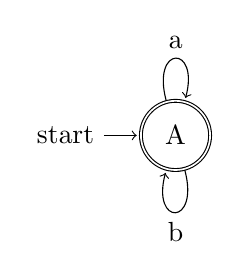
\begin{tikzpicture}[shorten >= 1pt, node distance = 2.5cm, on grid, auto]
  \node[state, initial, accepting] (A) {A};
  \path[->]
    (A) edge [loop above] node {a} (A)
        edge [loop below] node {b} (A);
\end{tikzpicture}
\end{document}
